\chapter{Jupter Notebook}
\section{简介}
\label{sec:jupyter_intro}
\reminder{\lefthand}{Jupyter Notebook 建议仅用于学习目的，不推荐用于项目开发。}
Jupter Notebook是基于网页的用于交互计算的应用程序。

其实Jupter Notebook与Jupter lab没什么大的区别

其功能
\begin{enumerate}[label=\arabic*)]
    \item 开发
    \item 运行代码
    \item 文档编写
    \item 展示结果
\end{enumerate}

\subsection{notebook 运行逻辑}
Jupyter Notebook不仅仅是一个简单的web应用程序，它还需要关联指定的kernel，用于执行我们的代码。

\begin{figure}[htpb]
  \centering
  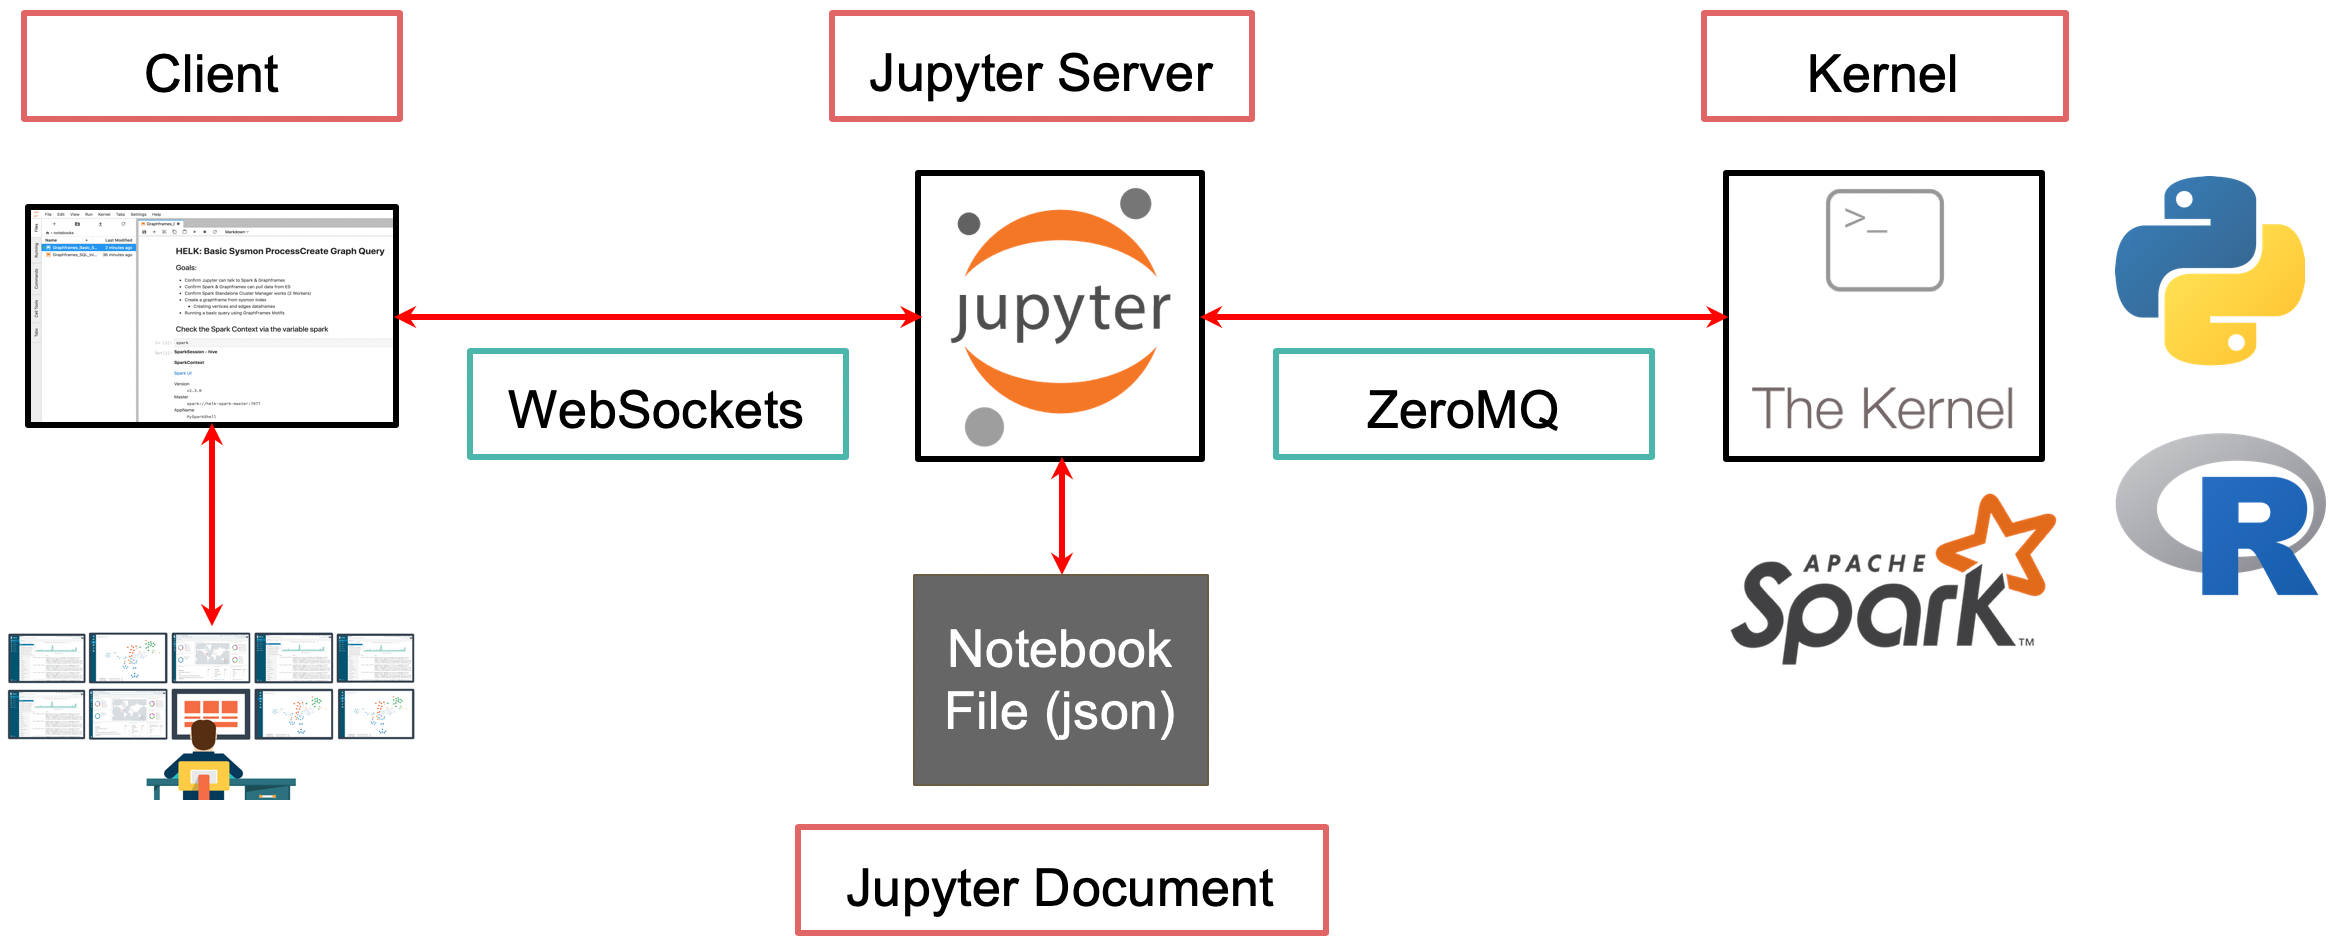
\includegraphics[width=0.6\textwidth]{part/软件工程/环境搭建/JupyterNotbook/pic/Jupyternotebook概述/jupyternotebook运行逻辑.png}
  \caption{Jupyter Notebook 运行逻辑}
  \label{fig:jupyternotebook运行逻辑}
\end{figure}

如图\ref{fig:jupyternotebook运行逻辑}所示，左边是用户写的代码，传输到中间的Jupyter server, server本身不能执行代码，server把代码传给Kernel，Kernel才是实际执行代码的组件，执行代码的地方。Kernel执行完代码，把结果返回给server，再返回到用户的网页。

Kernel不仅可以是python.exe，也可以是其他语言的解释器，如Julia, R等，更多kernel可以看支持的\href{https://github.com/jupyter/jupyter/wiki/Jupyter-kernels}{kernel列表}.

在pytorch开发中，kernel其实就是某一个python解释器——python.exe，我们需要为当前的notebook配置相应的kernel，来进入相应的虚拟环境，这样才能运行代码。

\section{安装}
\subsection{安装IPython(非必须)}
\begin{lstlisting}[style=demostyle,numbers=none]
# 安装
conda install ipython
# 或
pip install IPython # 安装IPython
\end{lstlisting}

\subsection{安装Jupyter}
\begin{lstlisting}[style=demostyle,numbers=none]
# 安装
conda install jupyter
# 或
pip install jupyter
\end{lstlisting}

\subsection{添加Kernel}
\begin{lstlisting}[style=demostyle,numbers=none]
# 1.进入虚拟环境
conda activate mypytorch
# 2.安装ipykernel工具包（安装jupyter）
conda install ipykernel
# 或
pip install ipykernel
# 3.为当前环境添加kernel
python -m ipykernel install --user --name=mypytorch
\end{lstlisting}

\subsection{代码补全}
\begin{lstlisting}[style=demostyle,numbers=none]
# 安装
pip install jupyter_contrib_nbextensions
## 有时会不匹配报错 pip install -i https://pypi.tuna.tsinghua.edu.cn/simple jupyter_contrib_nbextensions

conda install -c conda-forge jupyter_contrib_nbextensions
\end{lstlisting}

\section{使用}
\subsection{本地使用}
在那个目录下打开命令行，打开jupyter lab以后就是那个目录。
\begin{lstlisting}[style=demostyle,numbers=none]
# 切换到目标目录
cd 目标目录
# 激活虚拟环境
conda activate jupyter_notebook
# 在命令行中输入
jupyter notebook
# 或
jupyter lab # (推荐)更加强大的版本
\end{lstlisting}
\begin{figure}[htbp]
    \centering 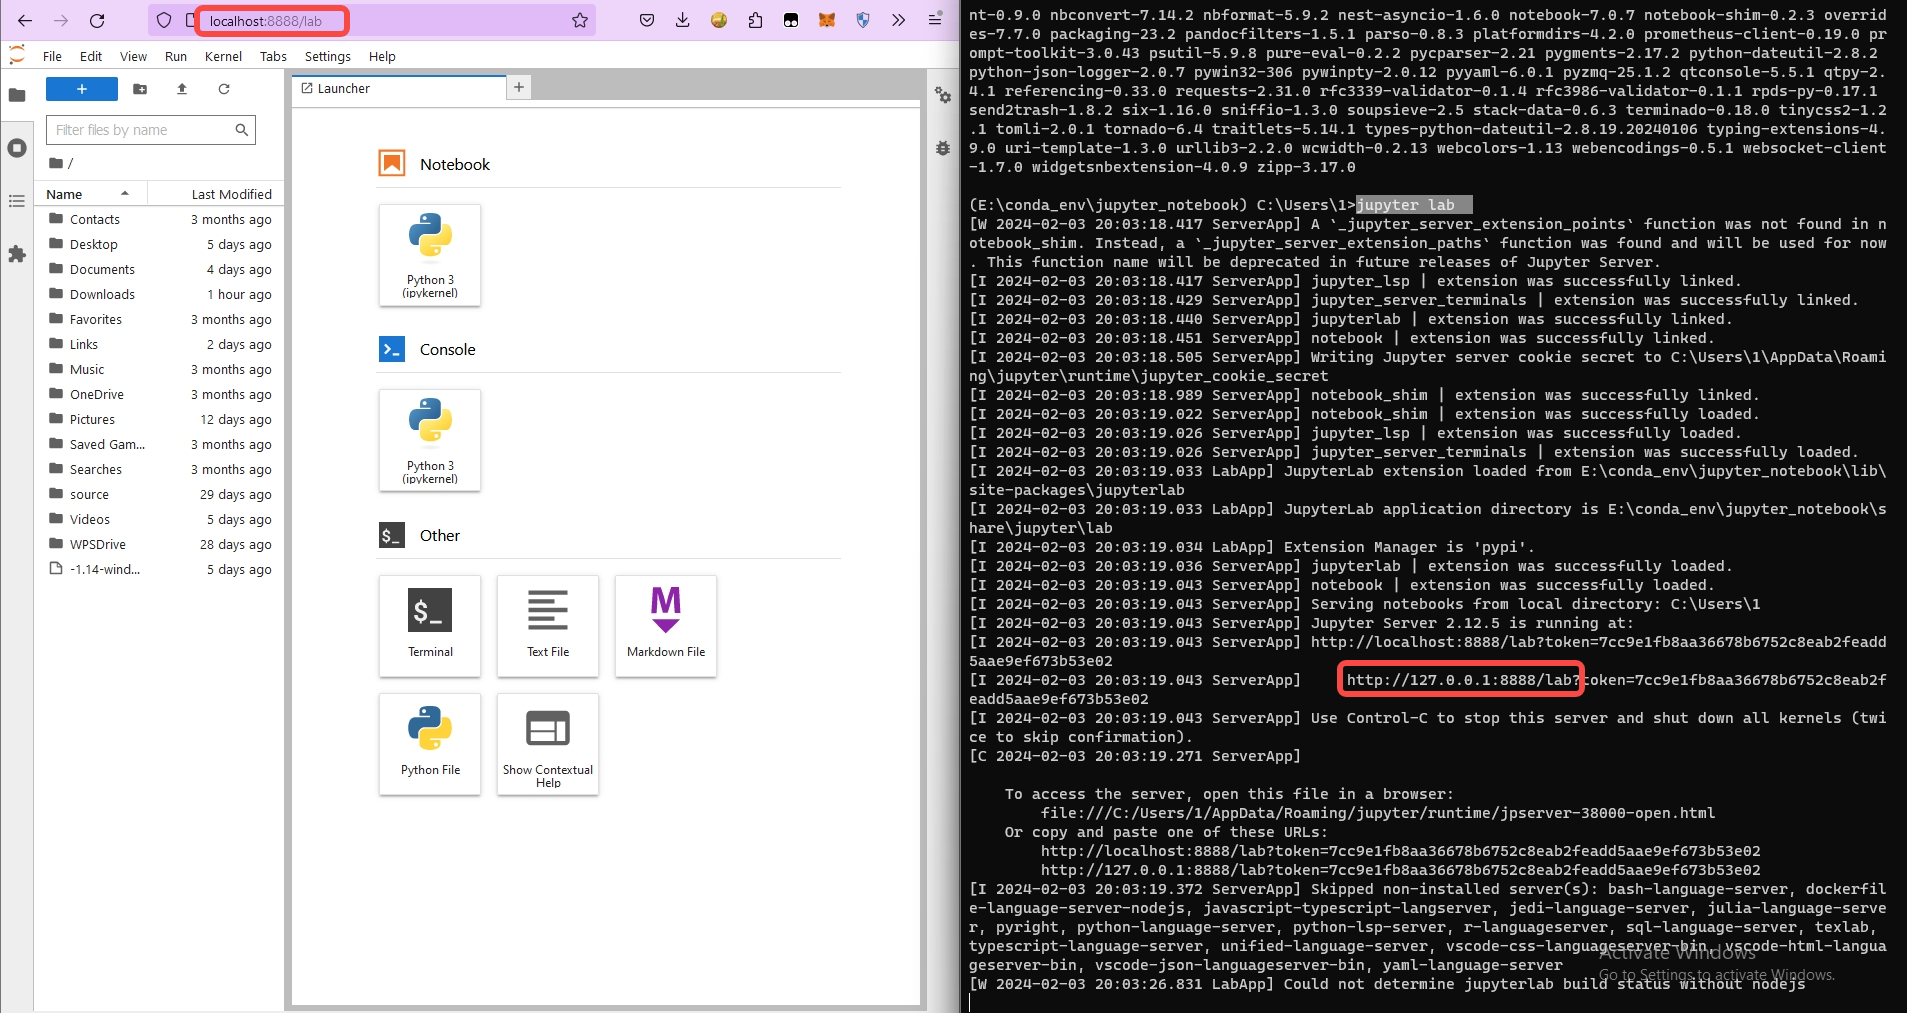
\includegraphics[width=.6\linewidth]{part/软件工程/环境搭建/JupyterNotbook/pic/Jupyternotebook概述/启动jupyter_lab.png}
      \caption{\label{fig:启动jupyter_lab}启动jupyter lab}
\end{figure}

\subsection{远程使用}
\subsubsection{远程服务器配置}
如图\ref{fig:配置远程连接JupterNotebook}所示，配置远程连接JupterNotebook。
\begin{lstlisting}[style=demostyle,numbers=none]
$(conda_env)> jupyter notebook --generate-config
Writing default config to: /home/tony/.jupyter/jupyter_notebook_config.py

(conda_env)> jupyter lab --generate-config
Writing default config to: /home/tony/.jupyter/jupyter_lab_config.py

$(conda_env)> vim ~/.jupyter/jupyter_notebook_config.py
c.NotebookApp.ip = '*'                     # 允许访问此服务器的 IP，星号表示任意 IP
c.NotebookApp.open_browser = False         # 运行时不打开本机浏览器
#c.NotebookApp.port = 8890                 # 使用端口，默认是 8888
c.NotebookApp.enable_mathjax = True        # 启用 MathJax
c.NotebookApp.allow_remote_access = True   #允许远程访问
#c.NotebookApp.allow_root = True           # 允许以root用户启动

$(conda_env)> jupyter notebook --no-browser --port=8888

$(conda_env)> jupyter lab --no-browser --port=8888
$(conda_env)> nohup jupyter lab --no-browser --port=8888 > $(date '+%Y-%m-%d-%H-%M-%S')-jupyter.log 2>&1 &
\end{lstlisting}

\begin{figure}[htbp]
    \centering 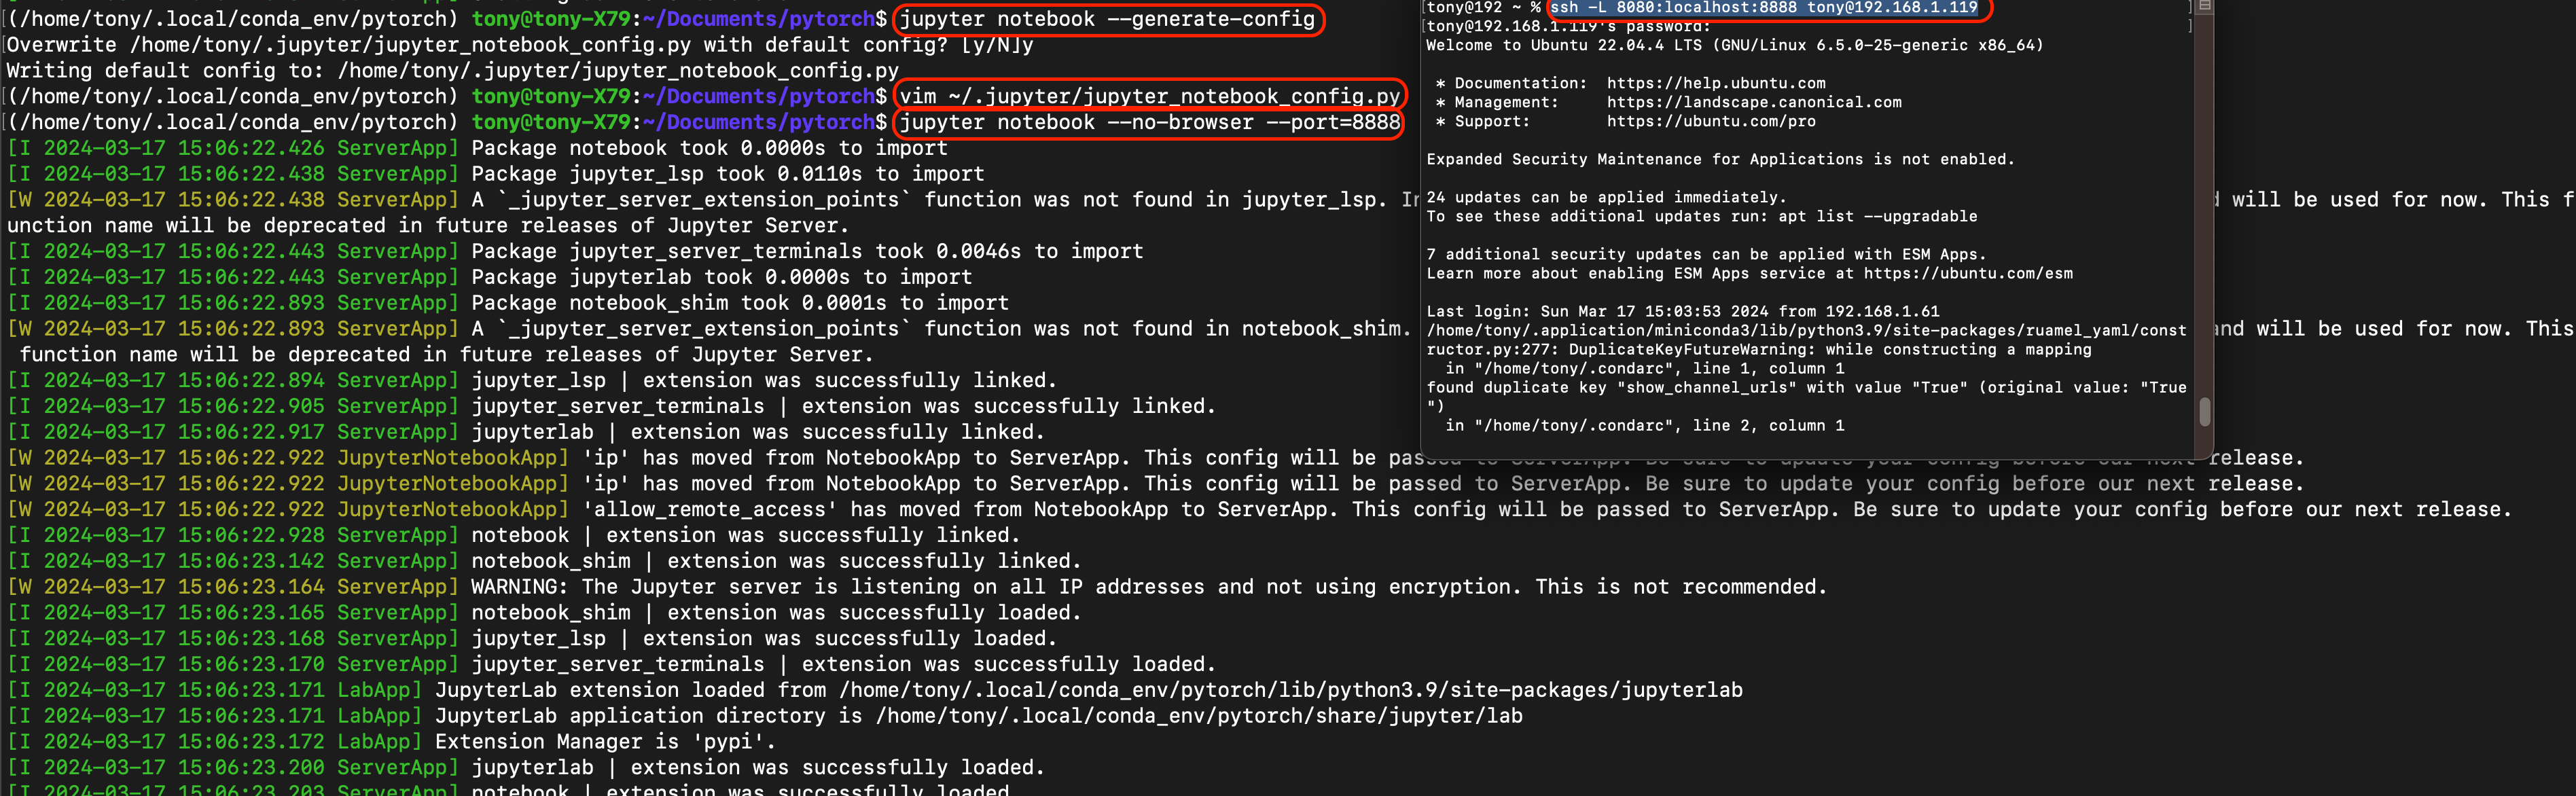
\includegraphics[width=.9\linewidth]{part/软件工程/环境搭建/JupyterNotbook/pic/Jupyternotebook概述/配置远程连接JupterNotebook.png}
      \caption{\label{fig:配置远程连接JupterNotebook}配置远程连接JupterNotebook}
\end{figure}

\subsubsection{本地访问远程JupterLab}
\subsubsubsection{配置防火墙访问}
\begin{lstlisting}[style=demostyle,numbers=none]
$(conda_env)> jupyter lab --no-browser --port=8888 # 在远程服务器上启动JupterLab
# 临时设置
$ sudo firewall-cmd --list-ports       # 列出所有开放都得端口
$ sudo firewall-cmd --add-port=8888/tcp # 添加临时的开放端口
$ sudo firewall-cmd --remove-port=8888/tcp # 关闭临时的开放端口

# 永久设置
$ firewall-cmd --list-ports --permanent # 查看所有永久开放的端口（默认为空）
$ sudo firewall-cmd --add-port=8888/tcp --permanent # 添加永久的开放端口
$ sudo firewall-cmd --remove-port=8888/tcp --permanent # 关闭永久的开放端口

# 配置结束后需要输入重载命令并重启防火墙以生效配置
$ sudo firewall-cmd --reload
$ sudo systemctl restart firewalld
\end{lstlisting}  

\begin{figure}[htbp]
  \centering 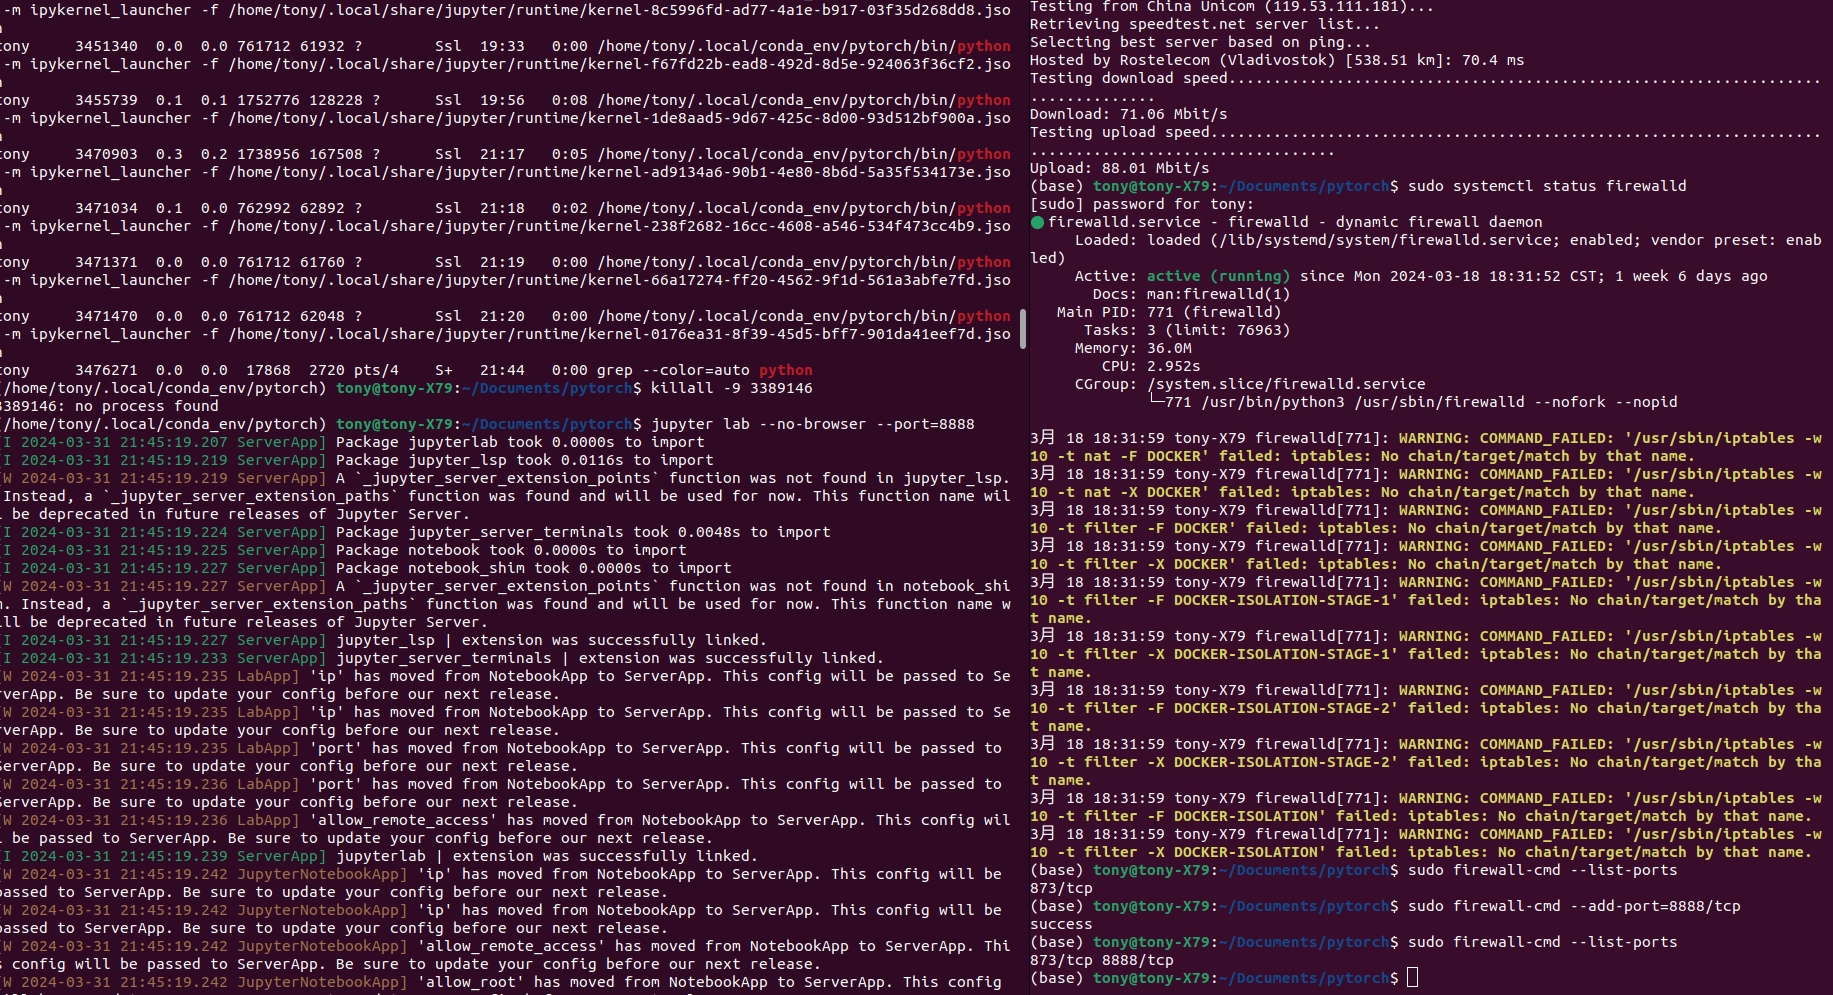
\includegraphics[width=.9\linewidth]{part/软件工程/环境搭建/JupyterNotbook/pic/Jupyternotebook概述/远程开启jupyter_lab防火墙.png}
    \caption{\label{fig:远程开启jupyterlab防火墙}远程开启jupyter lab防火墙}
\end{figure}

\begin{figure}[htbp]
  \centering 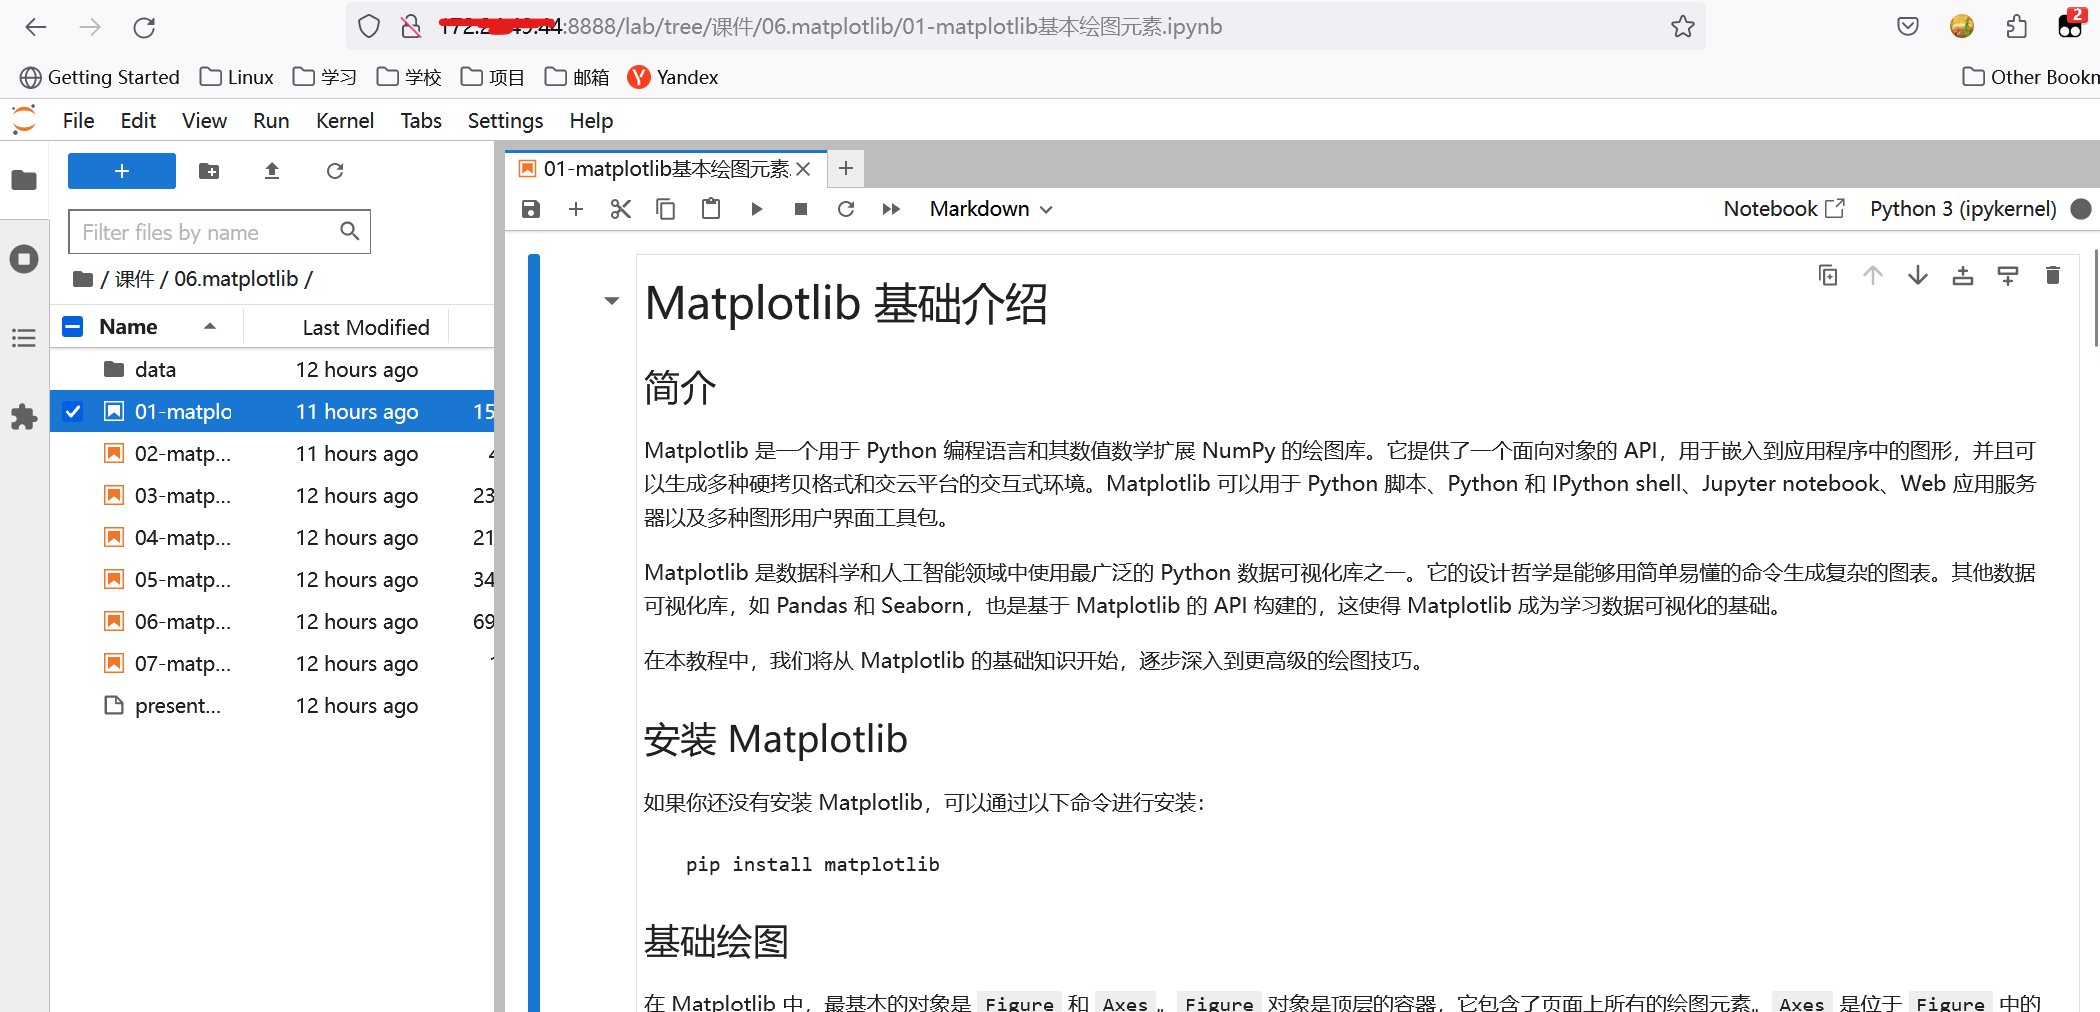
\includegraphics[width=.9\linewidth]{part/软件工程/环境搭建/JupyterNotbook/pic/Jupyternotebook概述/配置防火墙访问JupterLab.png}
    \caption{\label{fig:配置防火墙访问JupterLab}配置防火墙访问JupterLab}
\end{figure}

\subsubsubsection{SSH端口转发}
配置完需要使用ssh的端口转发(-L)功能，将远程的端口转发到本地(8080)，然后在本地访问即可,如图\ref{fig:访问远程JupterLab}所示。

\begin{lstlisting}[style=demostyle,numbers=none]
# ssh -L [本地端口]:localhost:[远程端口] [远程用户名]@[远程IP] -p [ssh连接端口]    
ssh -L 8080:localhost:8888 tony@192.168.1.119
\end{lstlisting}

\begin{figure}[htbp]
    \centering 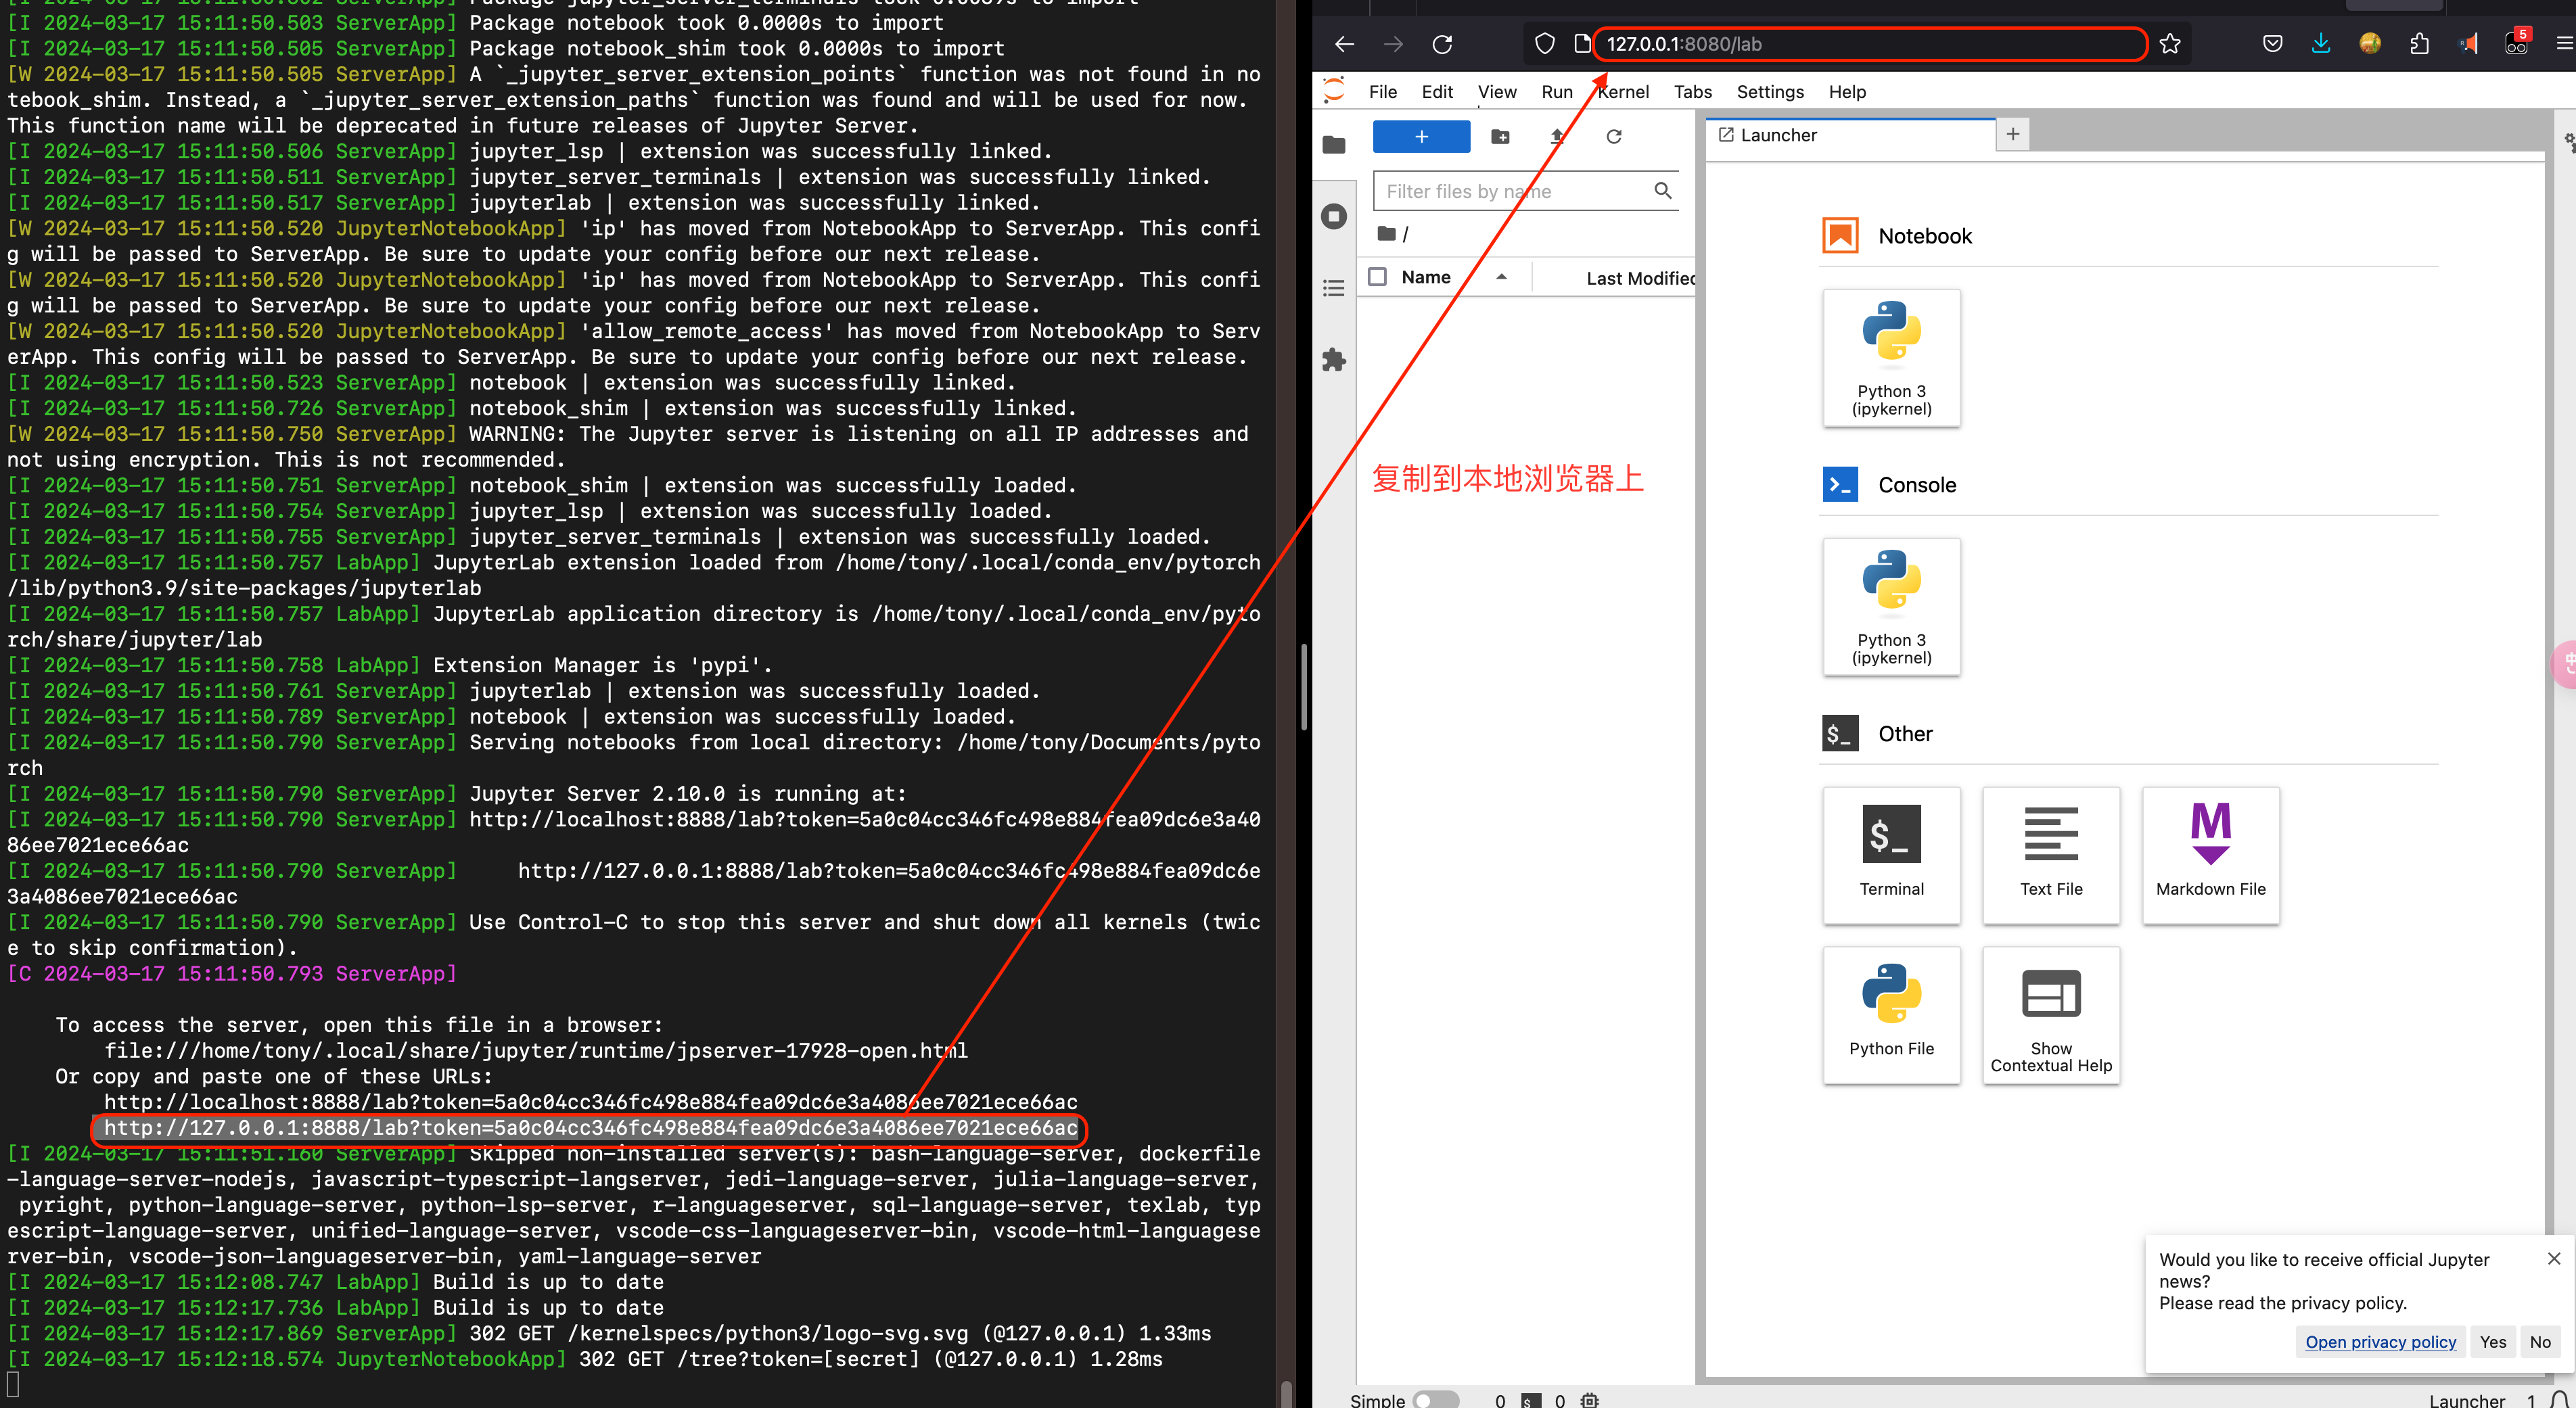
\includegraphics[width=.9\linewidth]{part/软件工程/环境搭建/JupyterNotbook/pic/Jupyternotebook概述/访问远程JupterLab.png}
      \caption{\label{fig:访问远程JupterLab}访问远程JupterLab,这里是localhost:8080}
\end{figure}

\subsubsubsection{配置密码}
按照如图\ref{fig:jupyterlab设置密码}所示设置密码。
\begin{figure}[htbp]
  \centering 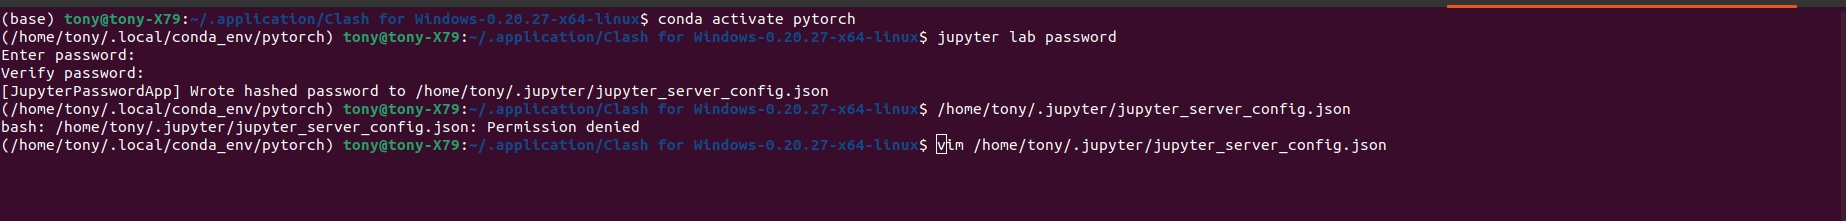
\includegraphics[width=.9\linewidth]{part/软件工程/环境搭建/JupyterNotbook/pic/Jupyternotebook概述/jupyterlab设置密码.png}
    \caption{\label{fig:jupyterlab设置密码}jupyterlab设置密码}
\end{figure}
然后按照如图\ref{fig:jupyterlab登入界面}所示登入。第一次登入需要输入密码，以后就不需要了。
\begin{figure}[htbp]
  \centering 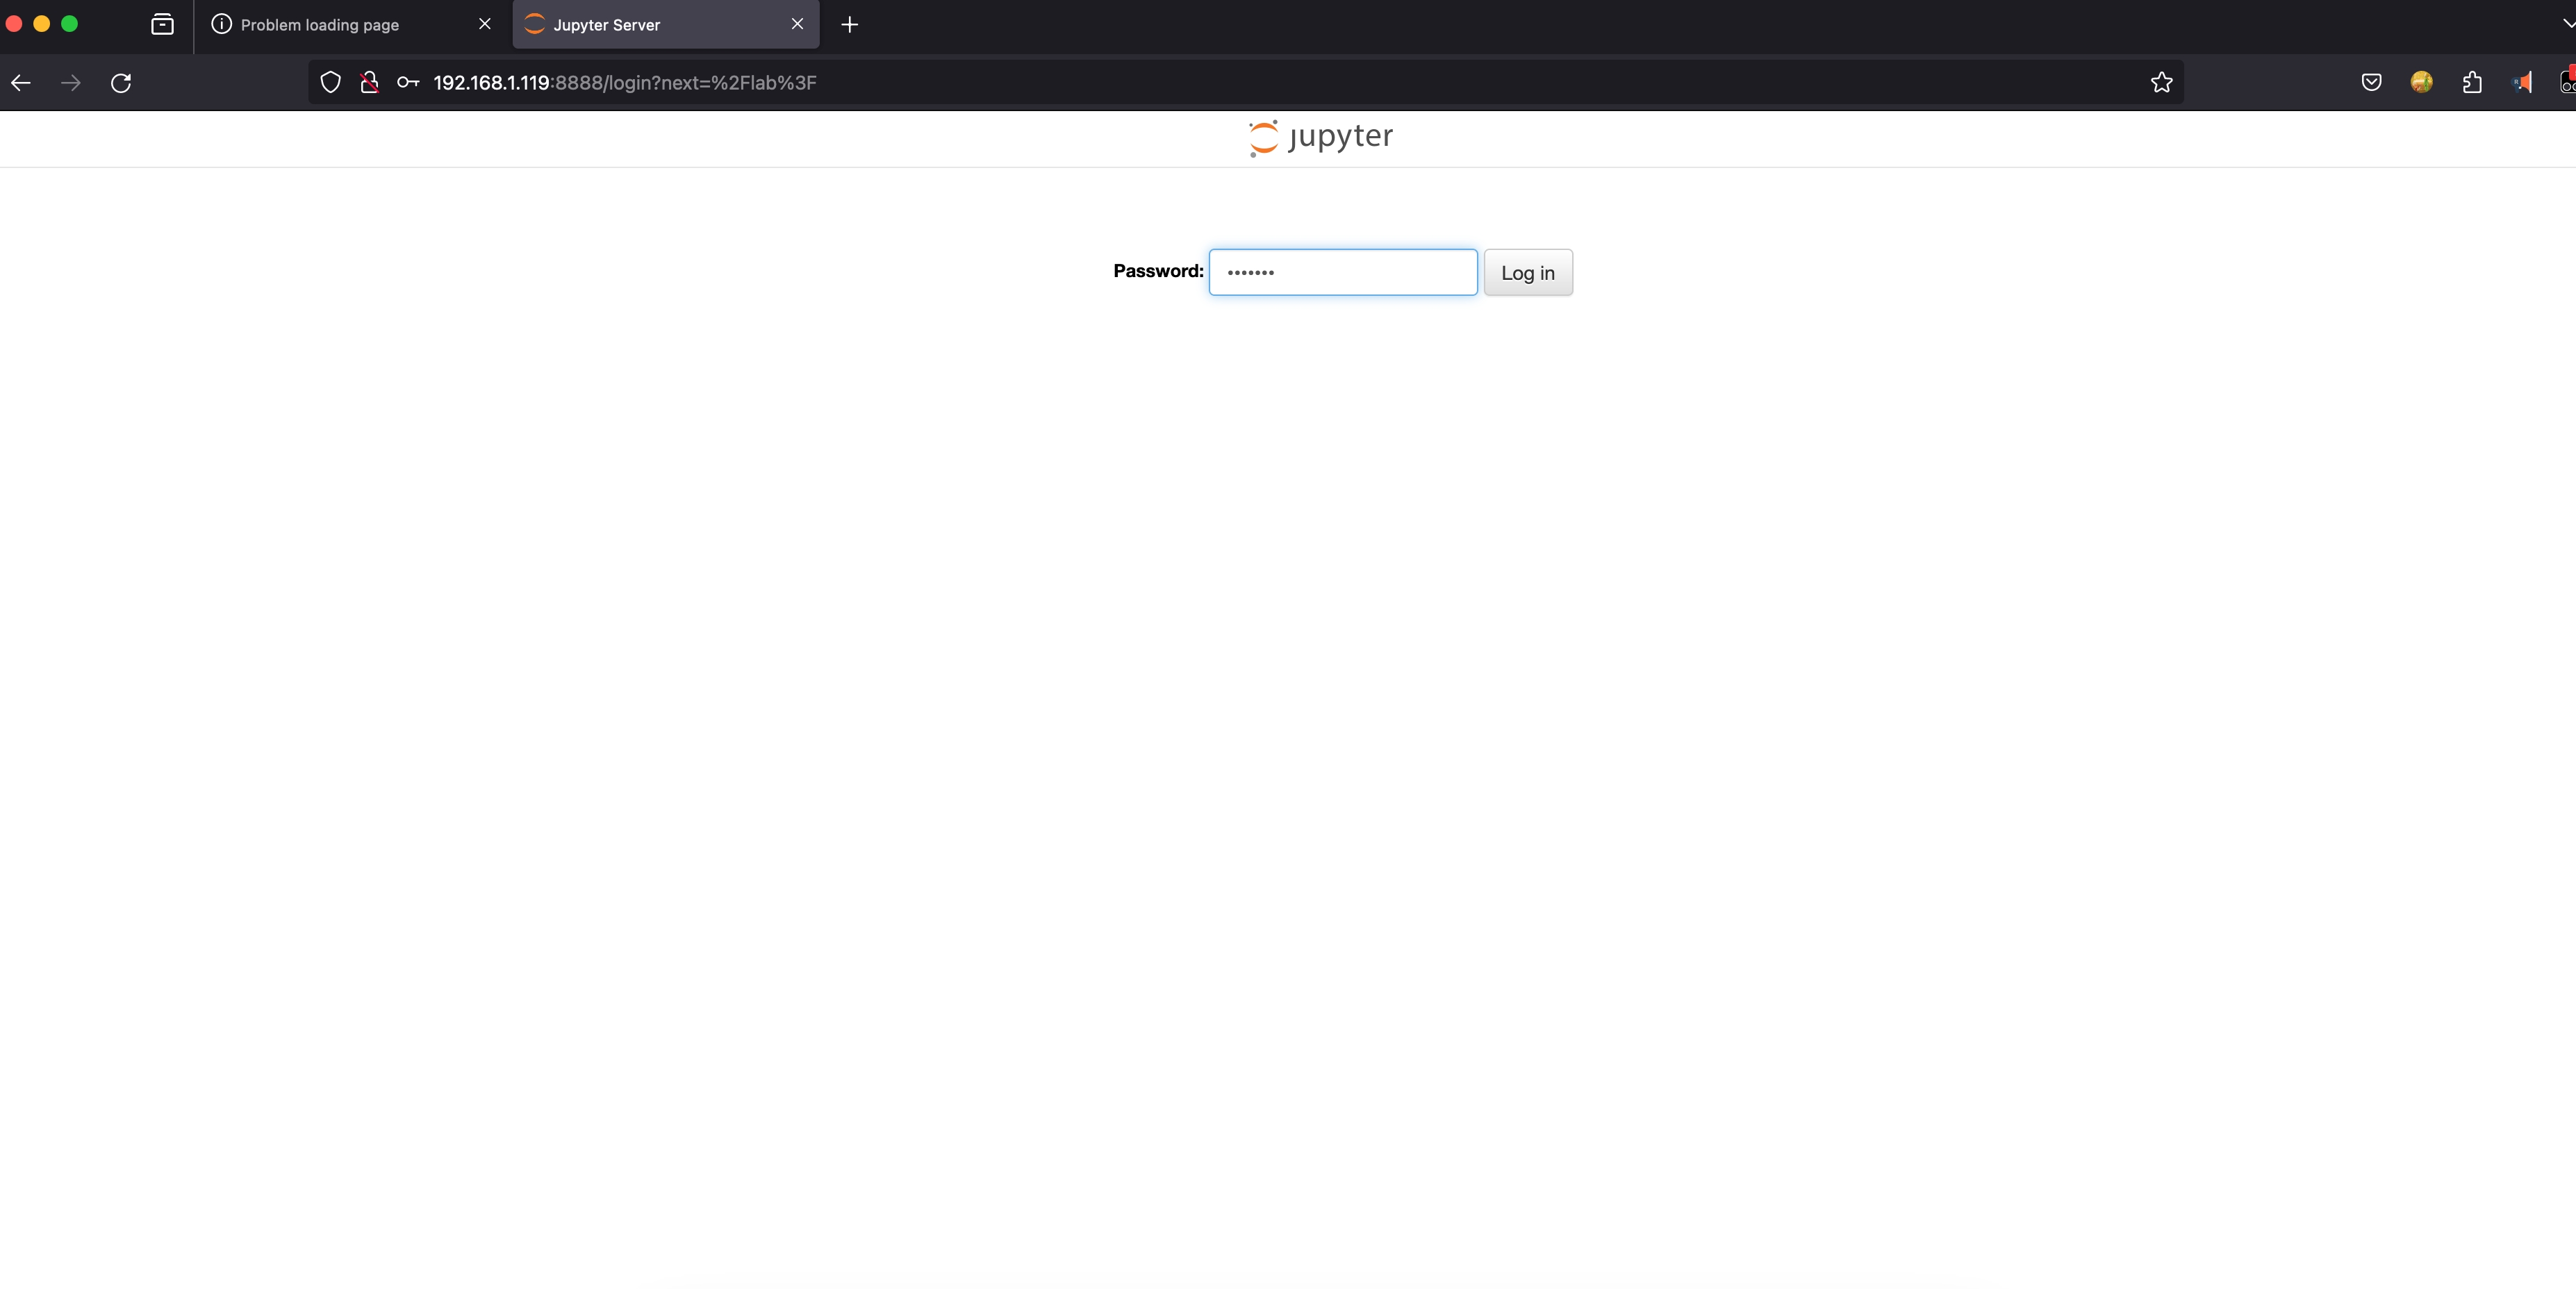
\includegraphics[width=.9\linewidth]{part/软件工程/环境搭建/JupyterNotbook/pic/Jupyternotebook概述/jupyterlab登入界面.png}
    \caption{\label{fig:jupyterlab登入界面}jupyterlab登入界面}
\end{figure}






